\setcounter{section}{24}
\section{Определения неориентированного и ориентированного графов, пути, (вершинно) простого пути,
рёберно простого пути. Связь вершинной и рёберной простоты. Определение цикла, рёберно простого цикла, (вершинно) простого цикла. Определение достижимости между вершинами, простота
пути. Определение связности.}
\textbf{Определение} \textit{Ориентированным графом} G называется пара G=(V,E), где V — множество вершин , а $E \subset V\times V$ — множество рёбер.
\\
\\
\textbf{Определение} \textit{Неориентированным графом} G называется пара G=(V,E), где V — множество вершин, а E $\subset$\{\{v,u\}:v,u$\in$V\} — множество рёбер. (Под \{v,u\} понимается неупорядоченная пара)
\\
\\
\textbf{Определение} \textit{Путём} в графе называется последовательность вида $v_0v_1...v_k$, где $e_i\in E$, $e_i = (v_{i-1},v_i)$
\\
\\
\textbf{Определение} Путь называется \textit{реберно-простым}, если в нем нет повторяющихся пар ребер
\\
\\
\textbf{Определение} Путь называется \textit{вершинно-простым}(простым), если в нем нет повторяющихся вершин 
\\
\\
\textbf{Замечание}\\
Если путь вершинно-простой, то он и реберно-простой
\\ $\blacktriangle \ $ Если путь вершинно-простой, то в нем нет повторяющихся вершин, значит, и повторяющегося ребра возникнуть не может, так как для того, чтобы возникло повторяющееся ребро, необходима пара повторяющихся вершин \ $\blacksquare$
\\
\\
\textbf{Определение} Цикл называется \textit{вершинно-простым} (простым), если в нем нет повторяющихся вершин (кроме начальной и конечной) 
\\
\\
\textbf{Определение} Цикл называется \textit{реберно-простым}, если в нем нет повторяющихся пар ребер
\\
\\
\textbf{Определение} Пусть u, v $\in V(G)$, тогда говорим, что из \textit{u достижима v}, если из u есть путь в v
\\
\\
\textbf{Замечание} Если из u есть путь в v,то из u есть простой путь в v
\\
$\blacktriangle $
\begin{center}
    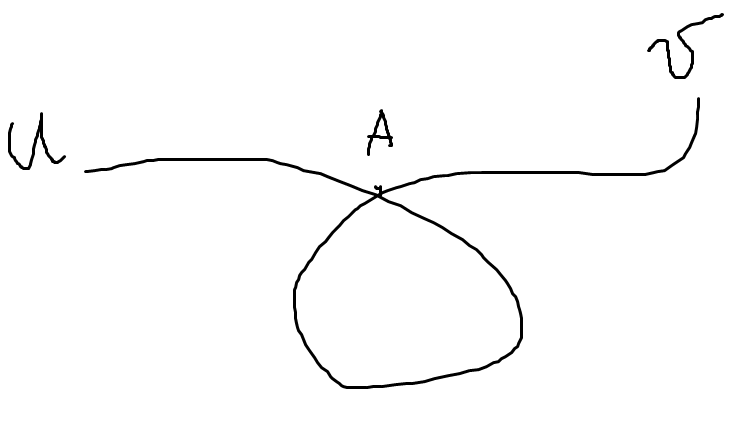
\includegraphics[width=8cm]{images/25-28_algo6.PNG}
\end{center}
Если пути пересекаются в какой-то точке A, можем игнорировать тот участок пути, который проходит от первого попадания в А на пути до последнего попадания в А, и пойти дальше до v. Таким образом можно избавиться от всех повторяющихся в пути вершин и сделать путь простым $\ \blacksquare$
\\
\\
\textbf{Определение} Неориентированный граф называется \textit{связным}, если между любыми двумя вершинами графа есть путь
\setcounter{section}{25}
\section{Три способа хранения графа в памяти компьютера, их преимущества и недостатки.}
\begin{itemize}
    \item [1] \textbf{Матрица смежности} 
    \begin{center}
        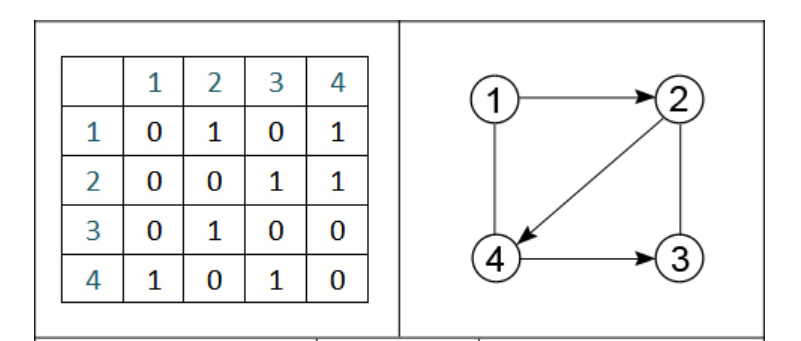
\includegraphics[width=8cm]{images/25-28_algo7.PNG}
    \end{center}
    - это матрица nxn, где n = |V|. На пересечении i строки и j столбца матрицы стоит 1 тогда и только тогда, когда в графе G есть ребро между вершиной i и вершиной j
    \begin{itemize}
        \item [+] За О(1) узнать, есть ли ребро между вершинами в графе
        \item [-] Занимает $n^2$ памяти
    \end{itemize}
     \item [2] \textbf{Список ребер} - просто хранить список ребер, как пары 
      \begin{itemize}
        \item [+] Более естественный способ задания
        \item [-] Неудобно работать. Не можем быстро проверить ни наличие ребра, ни узнать степень вершины и т.д.
    \end{itemize}
    \item [3] \textbf{Список смежности} - храним массив из n элементов $l_1,....,l_n$, где $l_i$ - список всех соседей вершины i
    \begin{itemize}
        \item [+] Хранится в памяти за O(n + m), так как всего у нас n списков, в которых суммарно не более 2m элементов
         \item [+] Знаем список соседей каждой вершины
        \item [-] Нельзя за O(1) узнать, есть ли ребро в графе (но можно использовать FixedSet, который занимает столько же памяти и позволяет узнать, есть ли ребро в графе. То есть этот минус можно обойти, использовав такую структурку)
    \end{itemize}
\end{itemize}
\setcounter{section}{26}
\section{Поиск в глубину: алгоритм dfs на ориентированном графе. Лемма о белых путях}
\begin{verbatim}
vector<vector<int>> g; \\ просто наш граф
vector<int> tin, tout; \\ время входа и выхода для каждой вершинки
int timer = 0;
vector<string> color(n, "white"); \\ будем красить вершины по мере посещения в три цвета
vector<int> parent;



void dfs(int v, int p = -1){
tin[v] = timer++; \\ заходим в в вершину, увеличиваем таймер
parent[v] = p; \\ проставляем родителя посещенной вершины
color[v] = "gray"; \\ красим вершину в цвет 1, помечая, что начинаем ее
                      использовать
for(int to: g[v]){ \\ выбираем, куда можно пойти из текущей вершины
    if(color[to]!= "white") continue; \\ если вершина, которую мы хотим посетить,
                                        уже начинала использоваться, ее цвет 
                                        не белый, то есть в нее мы пойти не
                                        можем
    dfs(to,v); \\ если вершина не использована, мы в нее идем
}
tout[v] = timer++; \\ перебрали все вершины, в которые можно попасть из v, 
                      записываем время выхода
color[v] = "black"; \\ помечаем, что вершина использована
}
\end{verbatim}
\textbf{Лемма о белых путях}
\\
Все пути, бывшие белыми в момент tin[v] и начинающиеся в v, станут черными в момент tout[v]
\\
$\blacktriangle \ $ Индукция в порядке убывания tin[v].
\begin{itemize}
    \item [1] База. tin[v] = max \\ Если tin[v] = max, то из вершины v в принципе нет белых путей. В противном случае мы пошли бы в какую-то вершинку впервые, и время входа в нее было бы больше, чем tin[v], что противоречит условию. Значит, к моменту tout[v] все пути из v будут покрашены в черный
    \item [2] Переход. Пусть есть какая-то вершина v и белый путь из нее к моменту времени tin[v]. 
    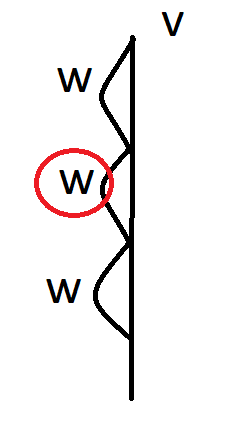
\includegraphics[width = 5cm]{images/25-28_фдп8.PNG}
    
    Пусть не все вершины из v к коменту времени tout[v] покрасилось в черный. Рассмотрим вершинку, которая будет самой верхней на пути из v, не покрашенной в черный. Пусть это вершина u. Рассмотрим вершину, которая выше u. Она покрашена в черный, значит, dfs перебрал все вершины, исходящие из нее, и в том числе он сходил в u, значит, u может быть только серой вершиной. Но и такого не может быть, поскольку для того, чтобы выйти из рекурсии на более высоком уровне(в вершине, из которой мы сходили в u) dfs должен выйти из рекурсии на более низком уровне, то есть, u должна покраситься в черный. Противоречие

    \begin{center}
        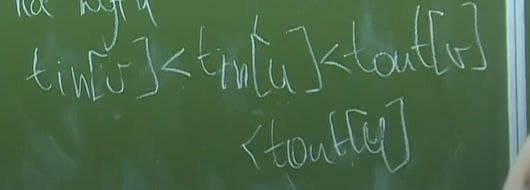
\includegraphics[width=8cm]{images/25-28_photo_2021-06-19_01-24-53.jpg}
    \end{center}
\end{itemize}
$\blacksquare$

\setcounter{section}{27}
\section{Поиск в глубину: множество посещаемых вершин, поиск цикла, достижимого из s, проверка на
ацикличность}
\textbf{Следствие} Из леммы о белых путях следует, что если вызвать dfs(s) из main, то все вершины, достижимые из s, посетятся
\\
$\blacktriangle \ $Это очевидно, поскольку изначально все пути белые, а значит, все пути, которые только можно пройти, будут покрашены в черный, то есть все достижимые вершины посетятся $\blacksquare$
\\
\\
\textbf{Следствие} В графе есть цикл, достижимый из s $\Longleftrightarrow$ dfs(s) когда-нибудь найдет ребро в color[to] = "gray"
\\
$\blacktriangle \;$
\begin{itemize}
    \item [$\rightarrow$] Пусть С - цикл, достижимый из s. Тогда при запуске dfs(s) мы обязательно посетим этот цикл. Пусть v - первая вершина цикла, которую мы посетим при обходе. Тогда к времени tin[v] весь остальной цикл еще белый, а значит, к моменту tout[v] мы пройдем весь цикл. В частности, посетится вершина u, являющаясь предыдущей для v в этом цикле. Значит, искомое ребро в серую вершину - (u,v).
    
    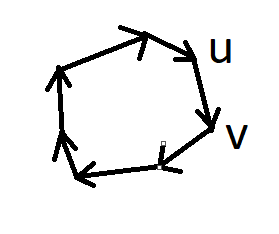
\includegraphics[width=5cm]{images/25-28_alg9.PNG}
    
    \item[$\leftarrow$] Стек рекурсии - это путь из серых вершин. Заметим, что наш dfs работает так:
     \begin{itemize}
         \item Запускаемся из s, красим ее в серый, перебираем ребра из нее. Выбираем какую-то вершинку, красим ее в серый и так далее 
        \begin{center}
             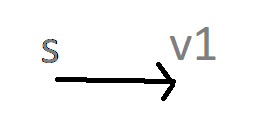
\includegraphics[width=4cm]{images/25-28_alg10.PNG}
             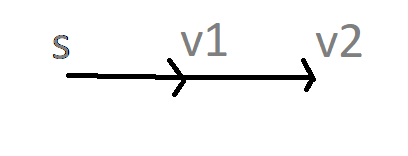
\includegraphics[width=6cm]{images/25-28_alg11.PNG}
             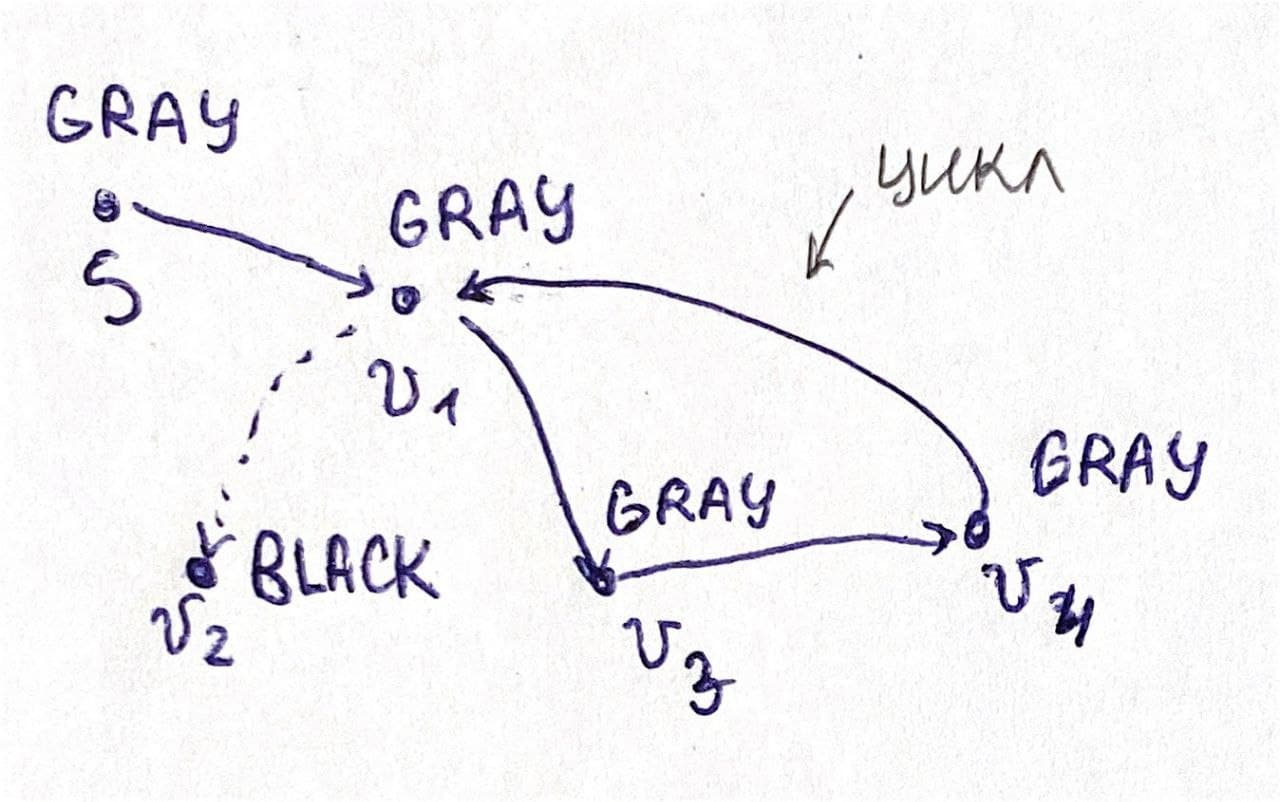
\includegraphics[width=5cm]{images/25-28_photo_2021-06-19_01-33-12.jpg}
        \end{center}
        \item Если мы походили-походили, не наткнулись на серую вершину и возвращаемся назад, вынимаем вершину из стека рекурсии и ищем новое ребро
        \begin{center}
             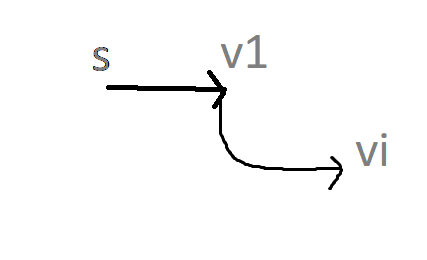
\includegraphics[width=7cm]{images/25-28_alg12.PNG}
        \end{center}
     \end{itemize}
     Отсюда следует, что если мы в какой-то момент наткнулись на серую вершину, то образуется цикл
\end{itemize}
$\blacksquare$\\
\textbf{Замечание}\\ Сам цикл можно восстановить, переходя по родителям до того момента, как мы окажемся в вершинке, откуда начался цикл \\
\\
\textbf{Определение} Граф называется \textit{ациклическим}(DAG - directed acyclic graph), если в нем нет циклов
\\
\\ 
Проверка графа на ацикличность совершается следующим образом. Произведём серию поисков в глубину в графе. Т.е. из каждой вершины, в которую мы ещё ни разу не приходили, запустим поиск в глубину, который будет искать цикл. Если цикл найден, возвращаем false. Если все вершины покрашены в черный, а цикл не найден - true